\documentclass{article}

\usepackage[margin=1in]{geometry}
\usepackage{graphicx}

\begin{document}
\title{Computer Design -- supervision 5}
\author{James Wood}
\maketitle

\section{Lecture 17}
\begin{enumerate}
  \item Multithreading allows the GPU to continue executing even if one batch of calculations stalls (waiting for IO, for example). Without multithreading, we would have to wait for the calculations to finish.
  \item To support multithreading, the GPU pipeline needs to have a scheduler. This manages which warp to run at a given time.
  \item A warp scheduler tries to keep to a round-robin schedule, but ignoring blocking threads.
  \item Each warp is given private registers, much as a regular CPU has registers. Each also has a local memory, which can shared between the threads on a single warp. The GPU also has a global memory, which can be used for sharing between all calculations happening. The shared forms of memory may be difficult to reason about (because concurrency usually is), but can safely be used for write-once data. Memories can also be slow, so there may be caches.
  \item Programs use GPUs well if they contain many independent computations that can happen at the same time as each other. As well as 3D graphics applications, numerical computing is often like this, particularly when working on large vectors. Programming languages like J and MATLAB can be used, where it is explicit in the program that certain array calculations work on each element of an array independently.
\end{enumerate}

\section{Lecture 18}
\begin{enumerate}
  \item Transistors can't get much smaller, so performance gains are coming from making multi-core machines. Having multiple cores requires more power, which generates more heat and inhibits performance.
  \item The big.LITTLE system has a collection of high-performance (big) cores with a collection of low-power (LITTLE) cores. The state is shared in such a way that switching between big and LITTLE cores doing the work is simple.
    \begin{enumerate}
      \item The intention is that the LITTLE cores do the work when not much is happening, and the computer switches to use the big cores when necessary.
      \item A third core type could be used, somewhere between the other two types in terms of power usage and performance. However, a similar effect can be achieved by using a mixture of big and LITTLE cores, and having medium cores would be wasteful in size and mass.
    \end{enumerate}
  \item It is possible to make special-purpose processors much more power-efficient than corresponding general-purpose processors. If there is a specific task occurring often, it may be worth making a specific processing unit for it to save power.
  \item Approximate computing can save energy at the expense of slightly incorrect results. This is useful particularly for problems with no good enough algorithm known to solve them.
\end{enumerate}

\section{Case study -- Intel Core i3-2350M (Sandy Bridge)}
\begin{itemize}
  \item Components: 2 cores, 2 cache layers, GPU, DMI 2.0 I/O bus
  \item x86\_64 instruction set, with AVX extension
  \item One level of per-core caches (256 KB each), one shared cache (3 MB), and maximum memory size of 16 GB
  \item Supports 4 hardware threads via hyperthreading
  \item Has Idle States, allowing idle cores to standby use less power
  \item 2.3 GHz clock speed on 32 nm lithography
  \item The mobile version has a slower clock speed than comparable desktop versions, contributing to its lower power usage and heat output.
  \item Has higher-frequency GPU, faster I/O bus, allows for more memory, and has higher memory bandwidth than Arrandale models. Ivy Bridge further improved amount and bandwidth of memory, and is smaller, with a feature size of 22 nm.
\end{itemize}
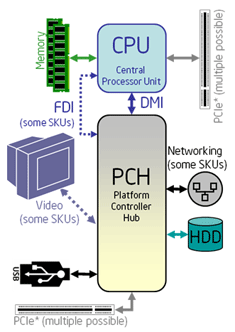
\includegraphics{diagram-18}

\end{document}
